\newpage
\section{Experiments}
\label{sec:AppendixB}

\subsection{Experiment 1}
    \begin{figure}[H]
        \centering
        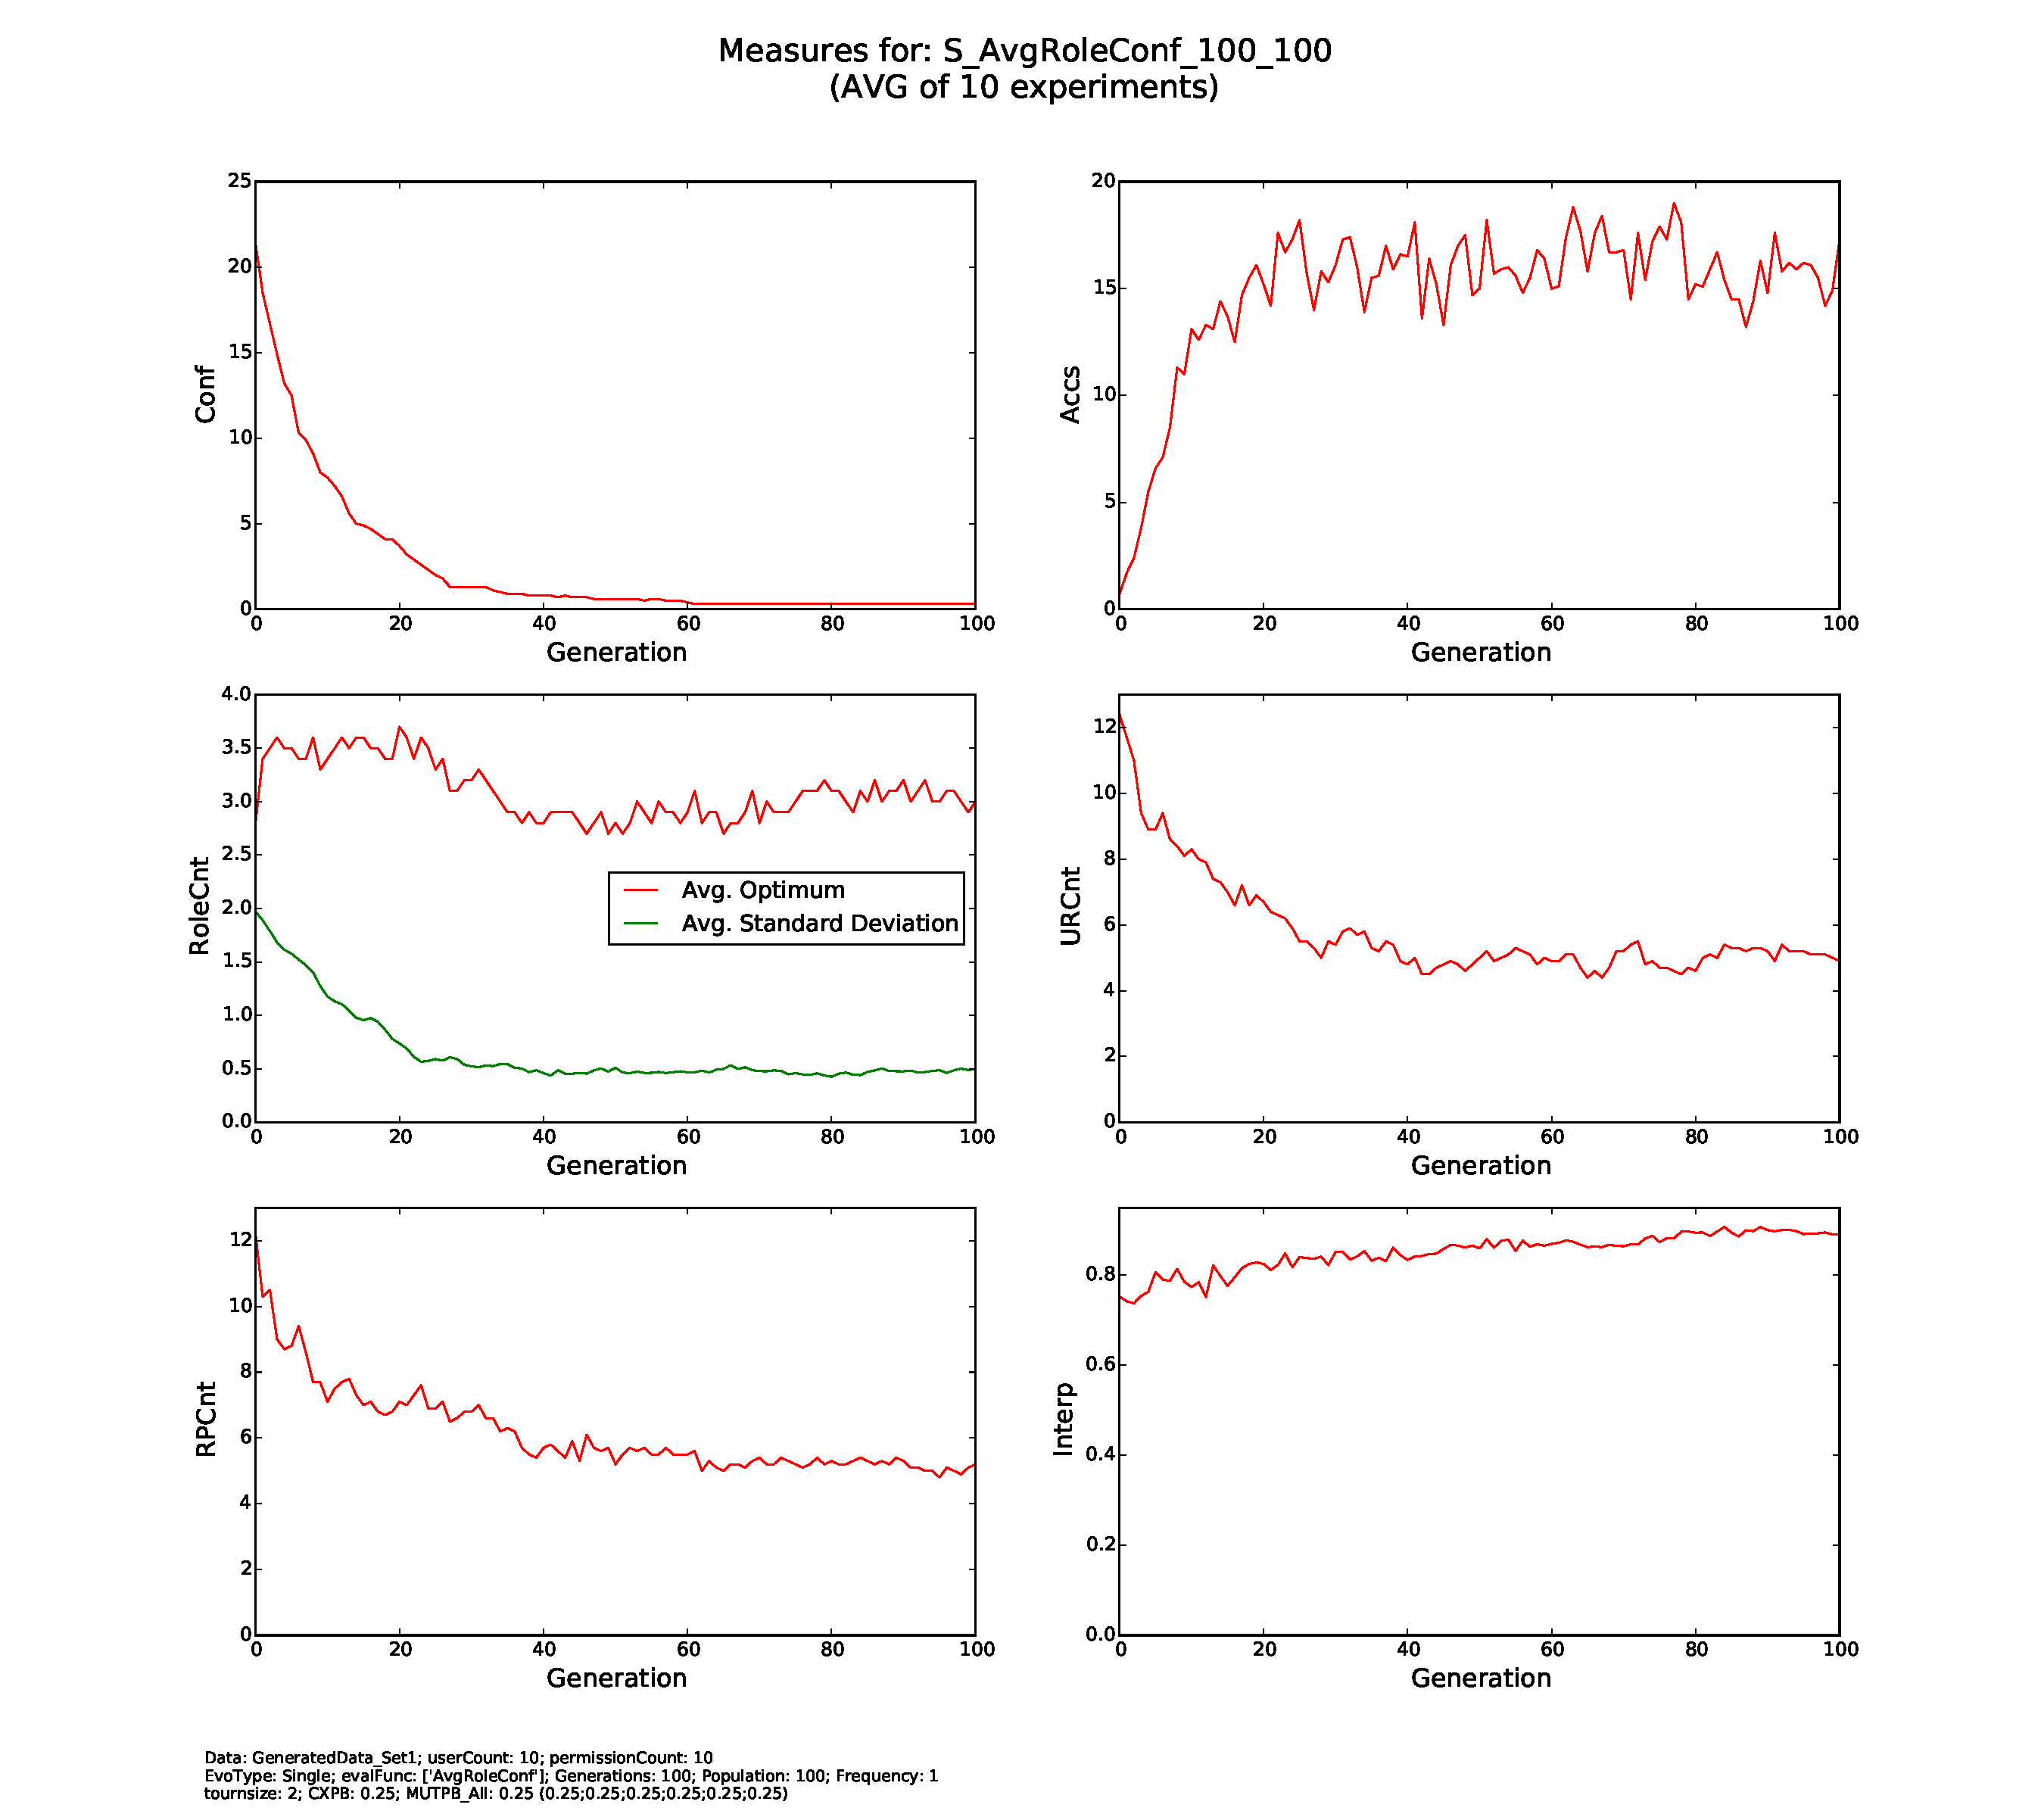
\includegraphics[scale=0.33, trim=4cm 2cm 4cm 0cm, clip=true]{./Figures/exp1avgConf}
        \caption{EXPERIMENT 1c: Results of EvoRoleMiner with Fitness function $F=avg(G_{conf})$ on synthetic dataset 1 with setup in table \ref{tab:setup1}. From u.l. to l.r.: Confidentiality Violations, Availability Violations, Role Count, User-Role Assignments, Role-Permission Assignments, Interpretability.}
        \label{fig:exp1avgConf}
    \end{figure}
    
    \begin{figure}[H]
        \centering
        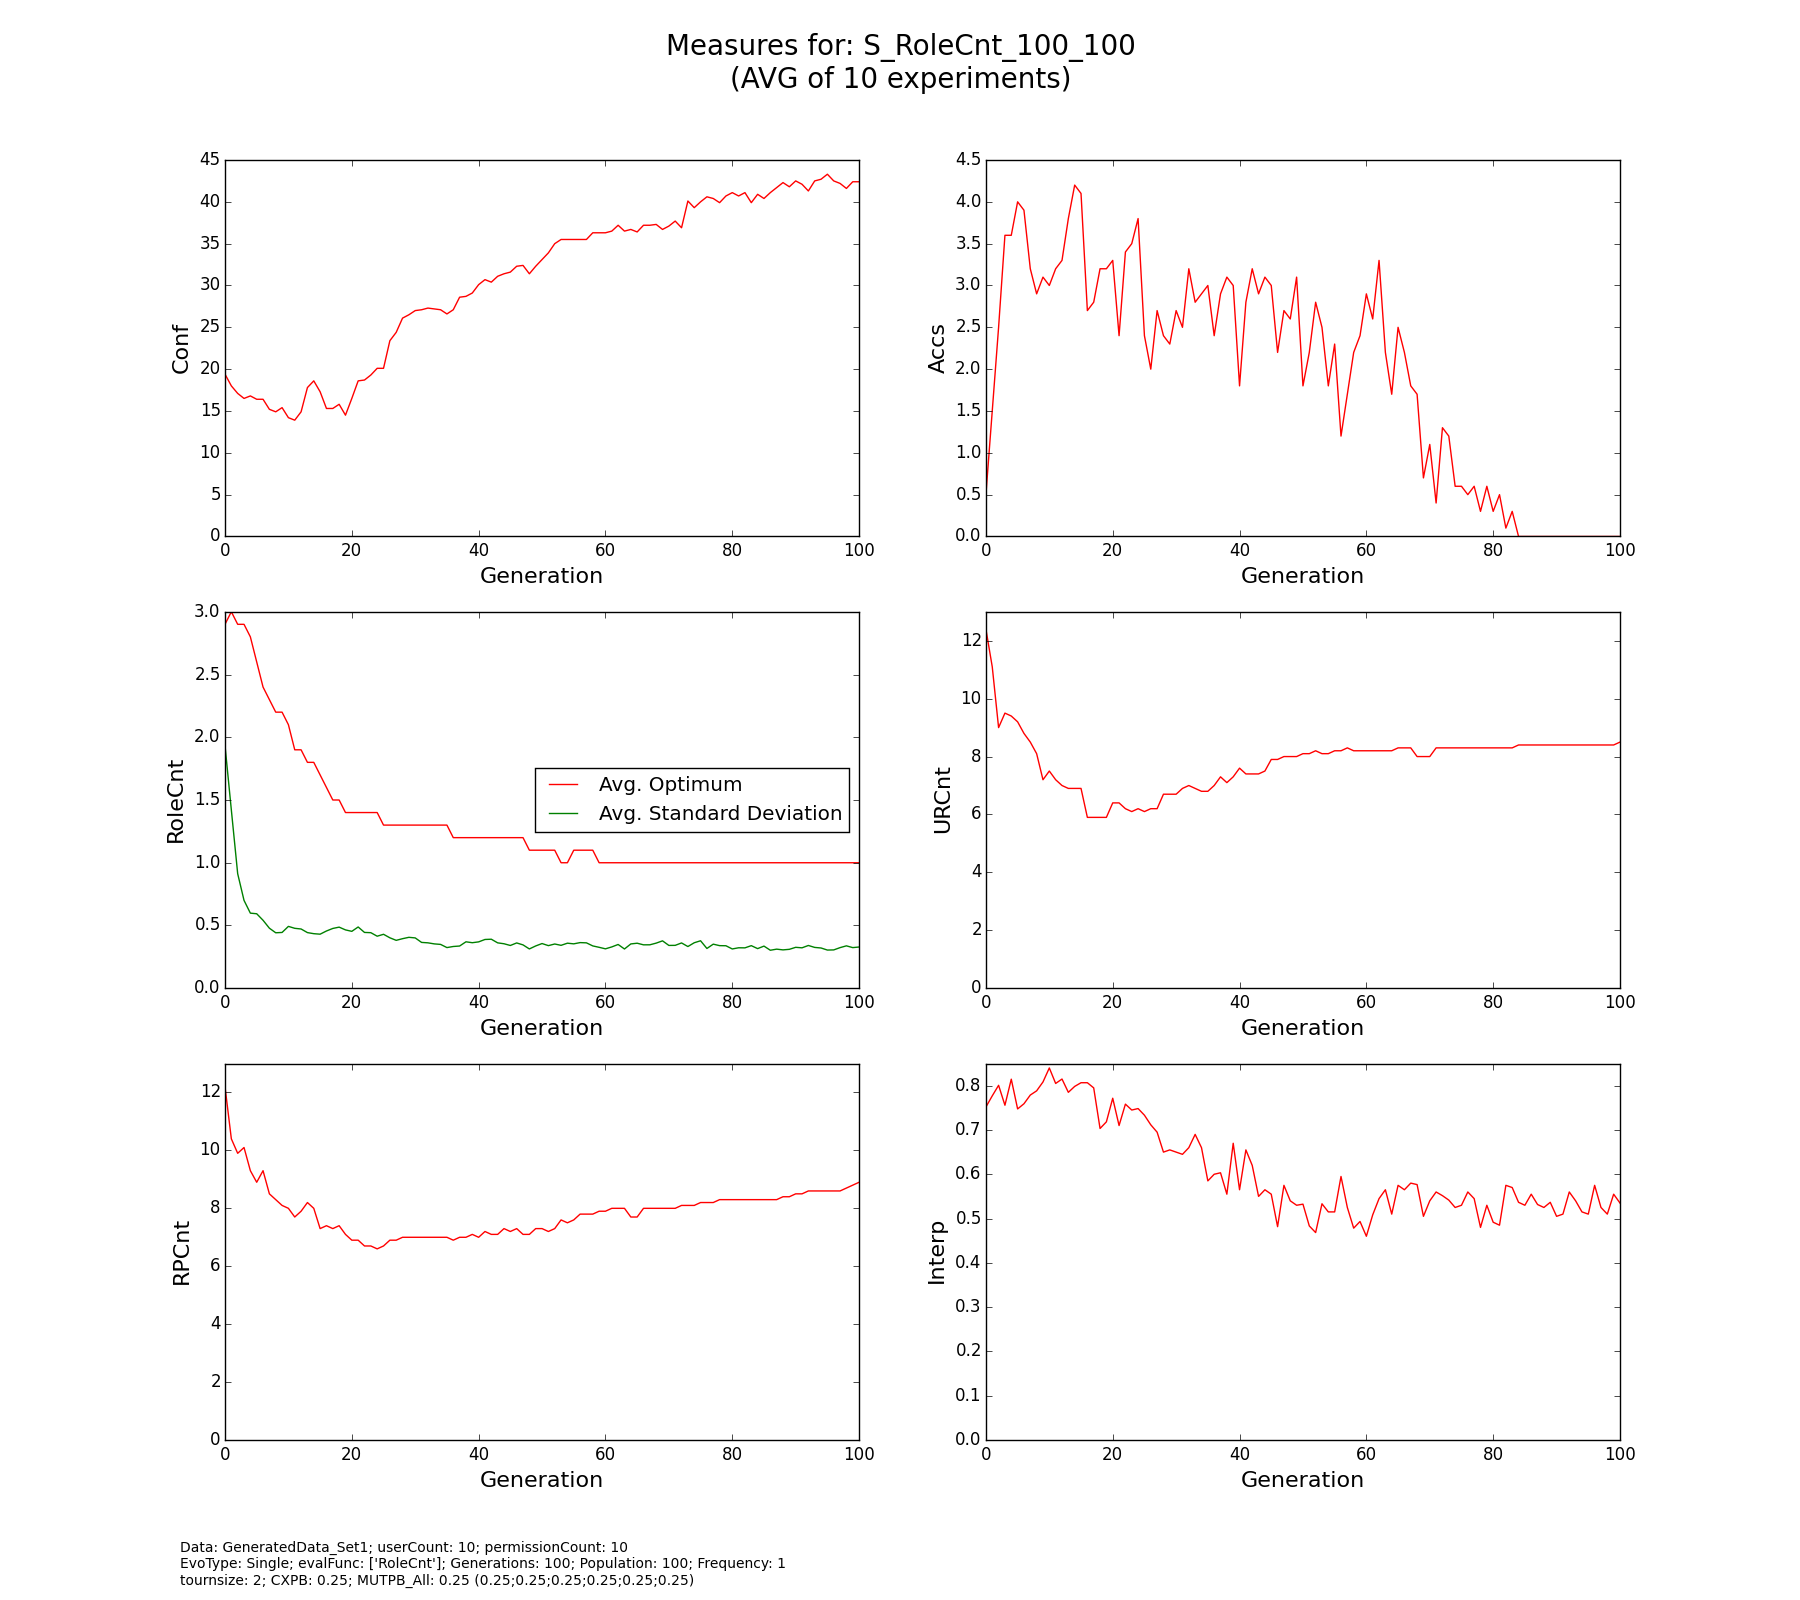
\includegraphics[scale=0.33, trim=4cm 2cm 4cm 0cm, clip=true]{./Figures/exp1roleCnt}
        \caption{EXPERIMENT 1d: Results of EvoRoleMiner with Fitness function $F=|R|$ on synthetic dataset 1 with setup in table \ref{tab:setup1}. From u.l. to l.r.: Confidentiality Violations, Availability Violations, Role Count, User-Role Assignments, Role-Permission Assignments, Interpretability.}
        \label{fig:exp1roleCnt}
    \end{figure}
    
    \begin{figure}[H]
        \centering
        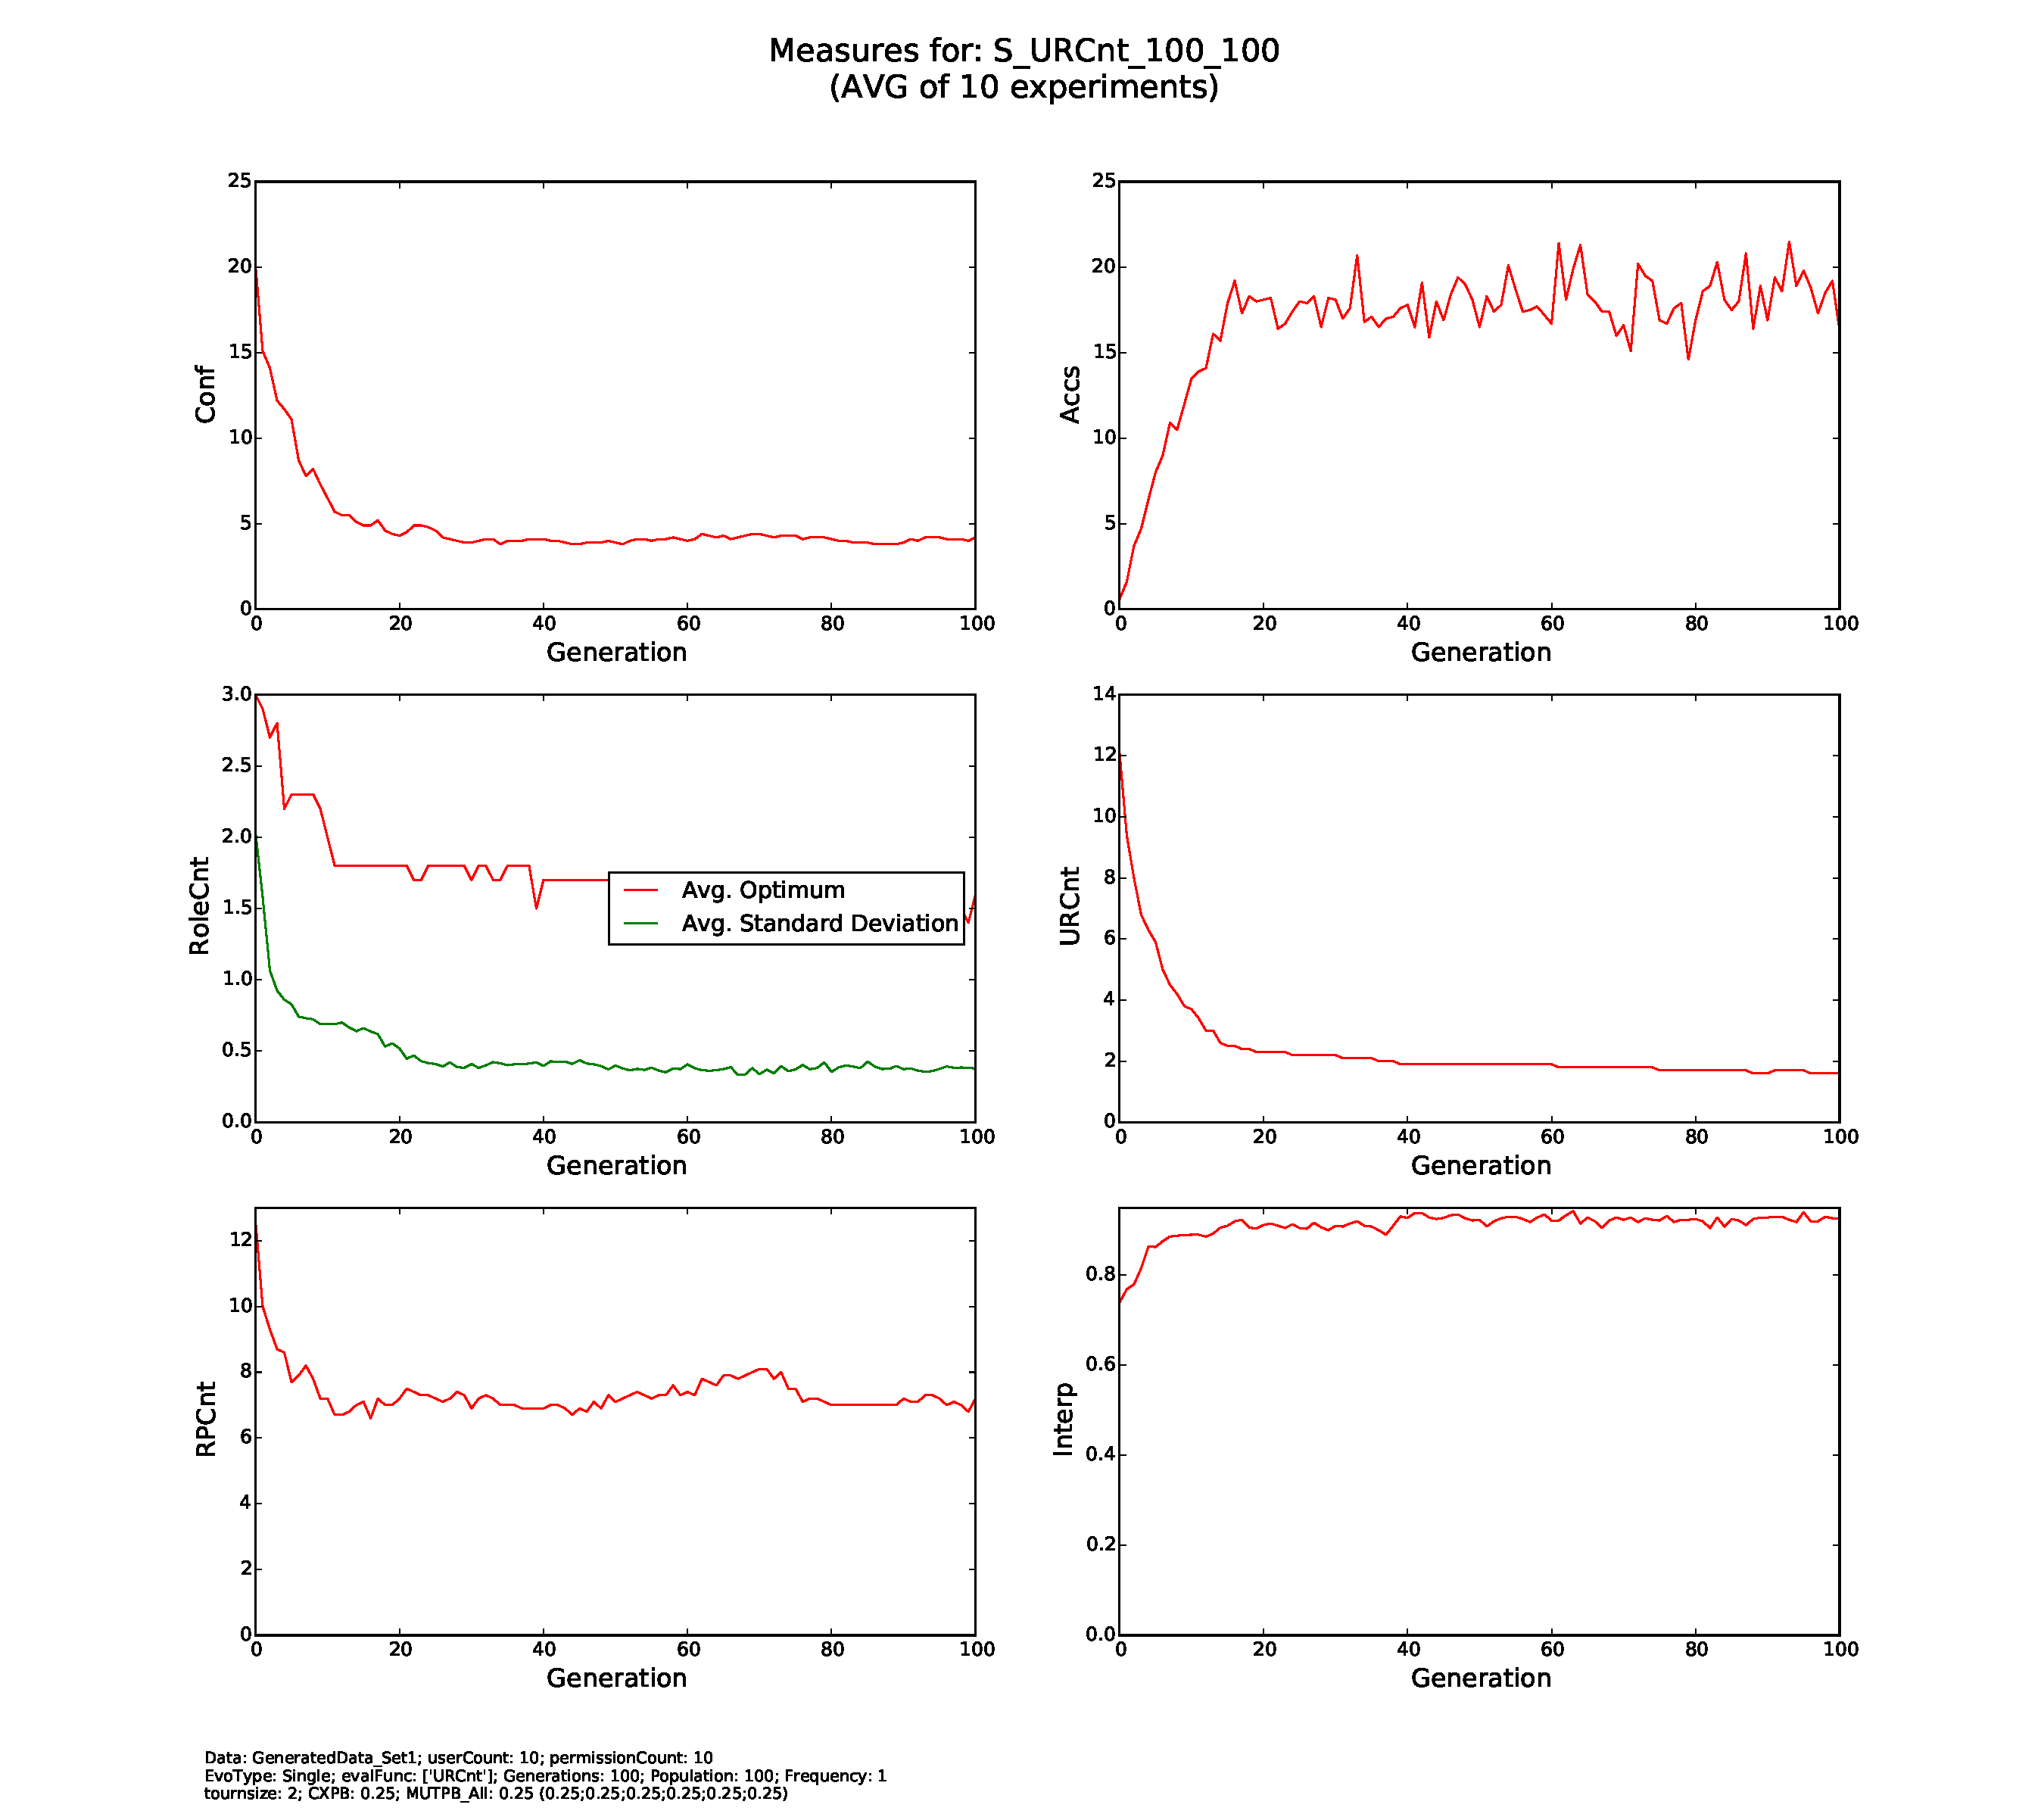
\includegraphics[scale=0.33, trim=4cm 2cm 4cm 0cm, clip=true]{./Figures/exp1urCnt}
        \caption{EXPERIMENT 1e: Results of EvoRoleMiner with Fitness function $F=|UA|$ on synthetic dataset 1 with setup in table \ref{tab:setup1}. From u.l. to l.r.: Confidentiality Violations, Availability Violations, Role Count, User-Role Assignments, Role-Permission Assignments, Interpretability.}
        \label{fig:exp1urCnt}
    \end{figure}
    
    \begin{figure}[H]
        \centering
        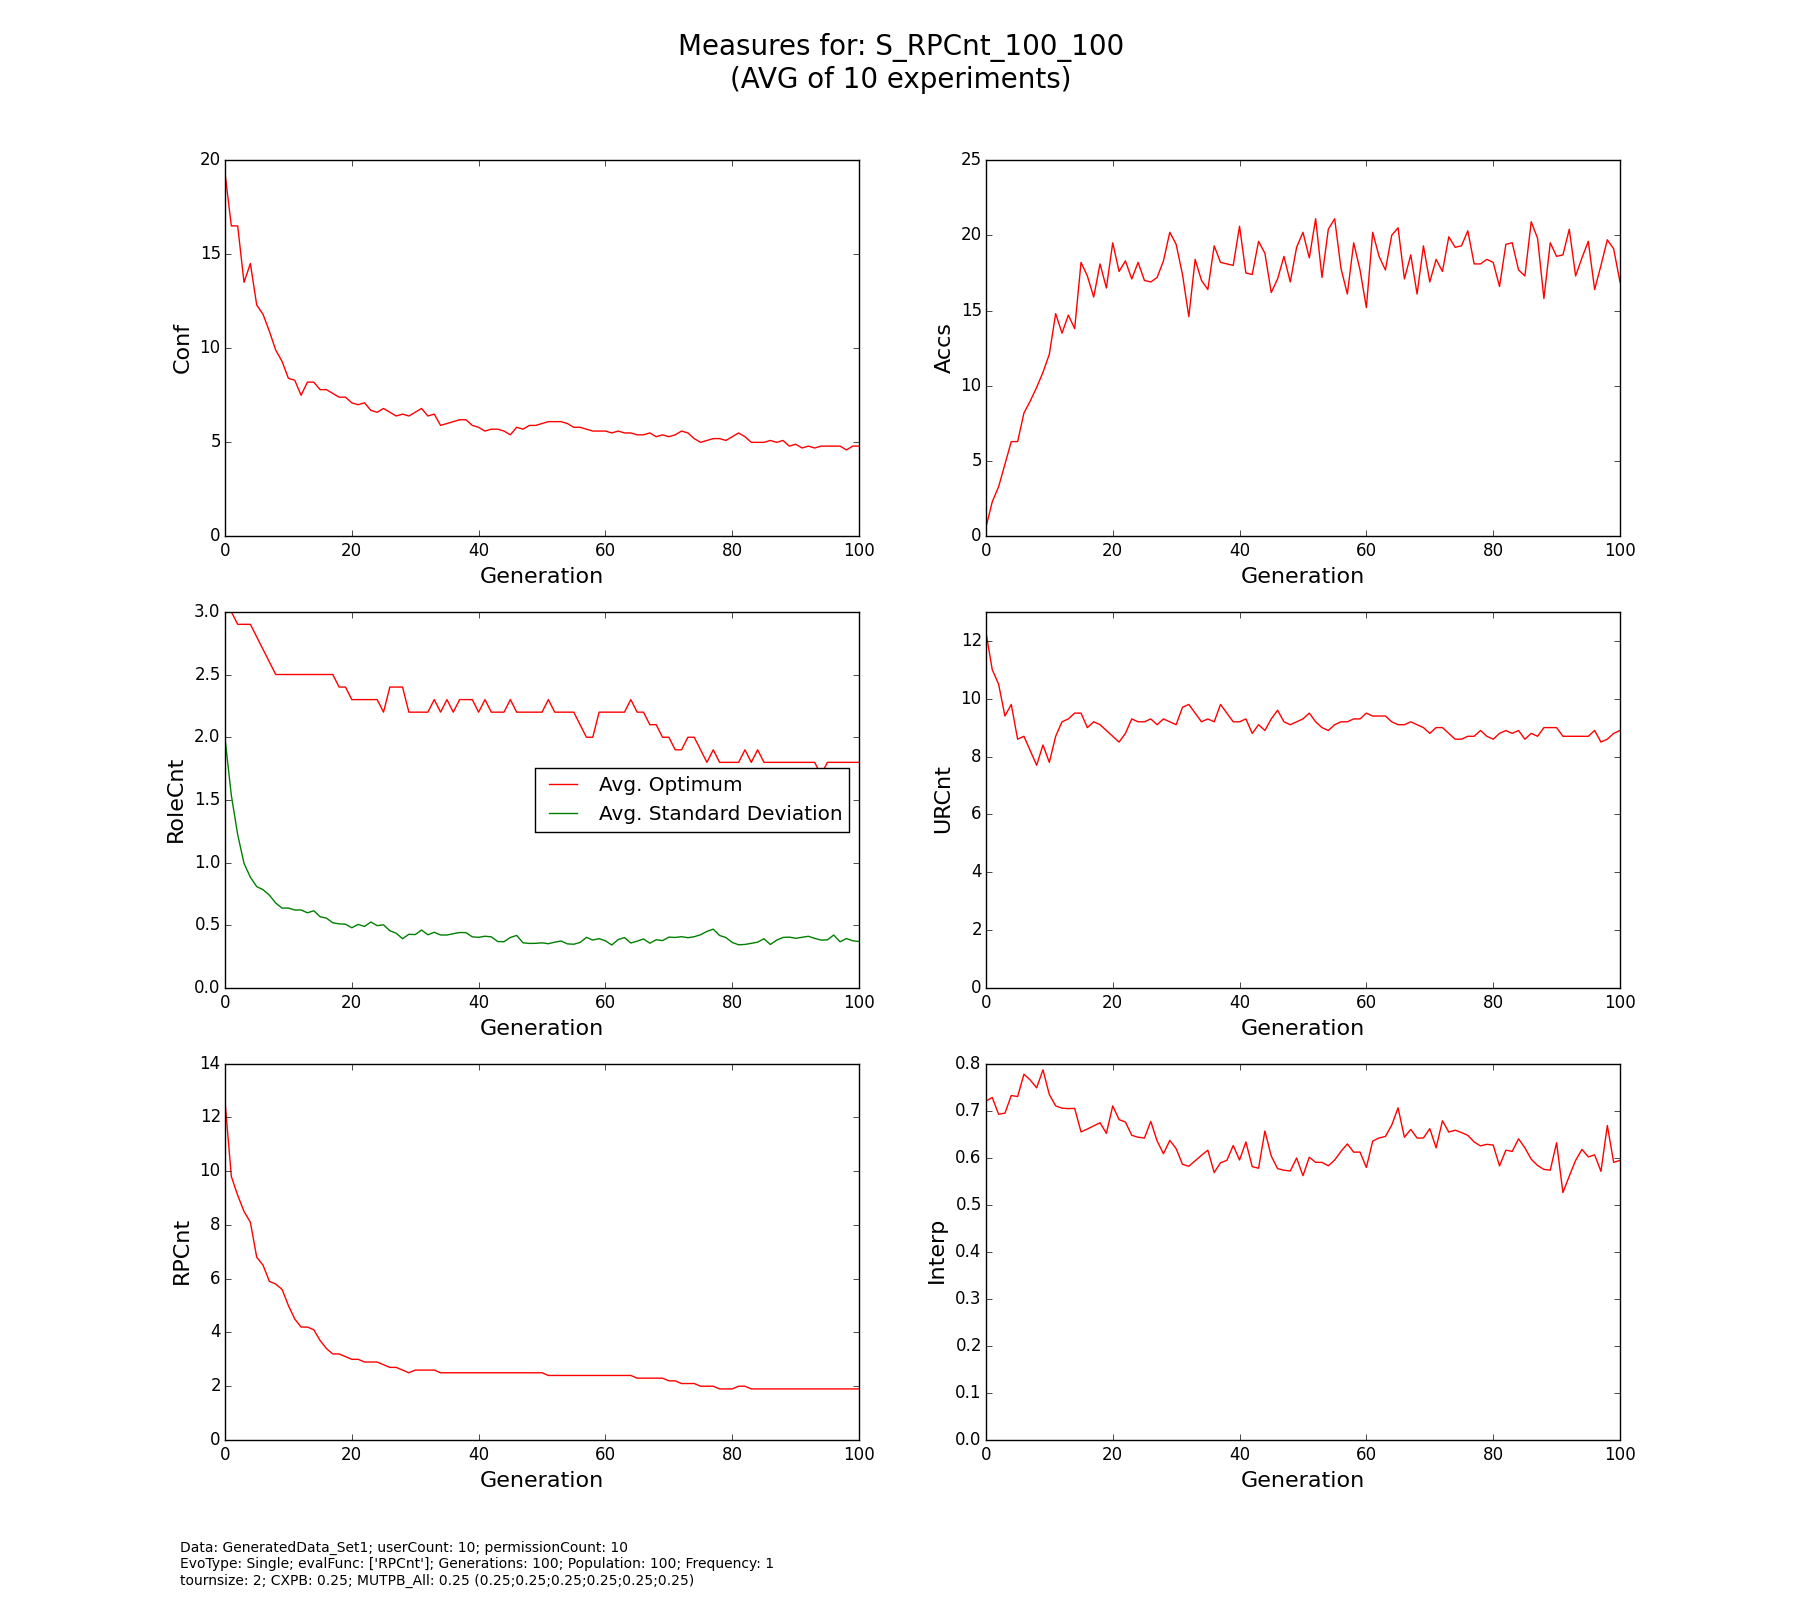
\includegraphics[scale=0.33, trim=4cm 2cm 4cm 0cm, clip=true]{./Figures/exp1rpCnt}
        \caption{EXPERIMENT 1f: Results of EvoRoleMiner with Fitness function $F=|PA|$ on synthetic dataset 1 with setup in table \ref{tab:setup1}. From u.l. to l.r.: Confidentiality Violations, Availability Violations, Role Count, User-Role Assignments, Role-Permission Assignments, Interpretability.}
        \label{fig:exp1rpCnt}
    \end{figure}

\subsection{Experiment 2a}
    \begin{figure}[H]
        \centering
        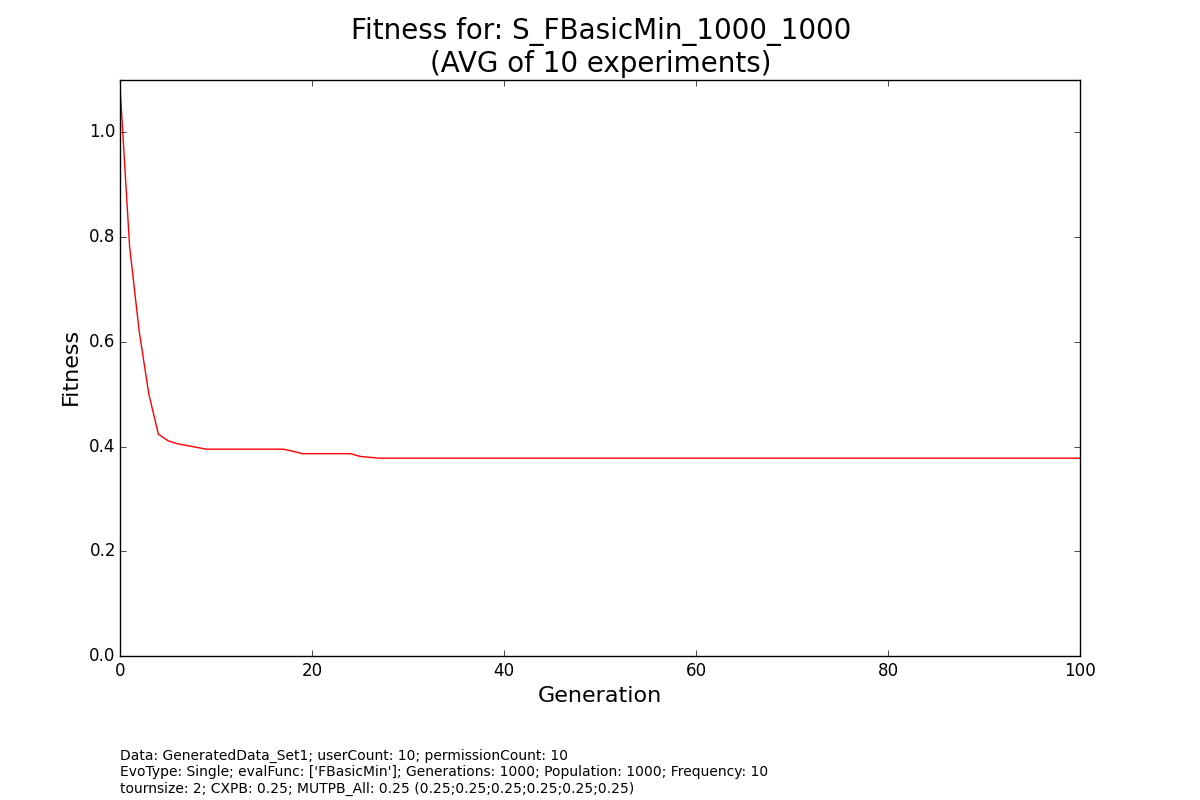
\includegraphics[scale=0.4, trim=0cm 2cm 0cm 0cm, clip=true]{./Figures/exp2aFitness}
        \caption{EXPERIMENT 2a: Average minimum Fitness Graph of ten experiments with fitness function $F_{basic}^{min}$ and synthetic dataset 1}
    \label{fig:exp2afitness}
    \end{figure}

    
\subsection{Experiment 2b}
    \begin{figure}[H]
        \centering
        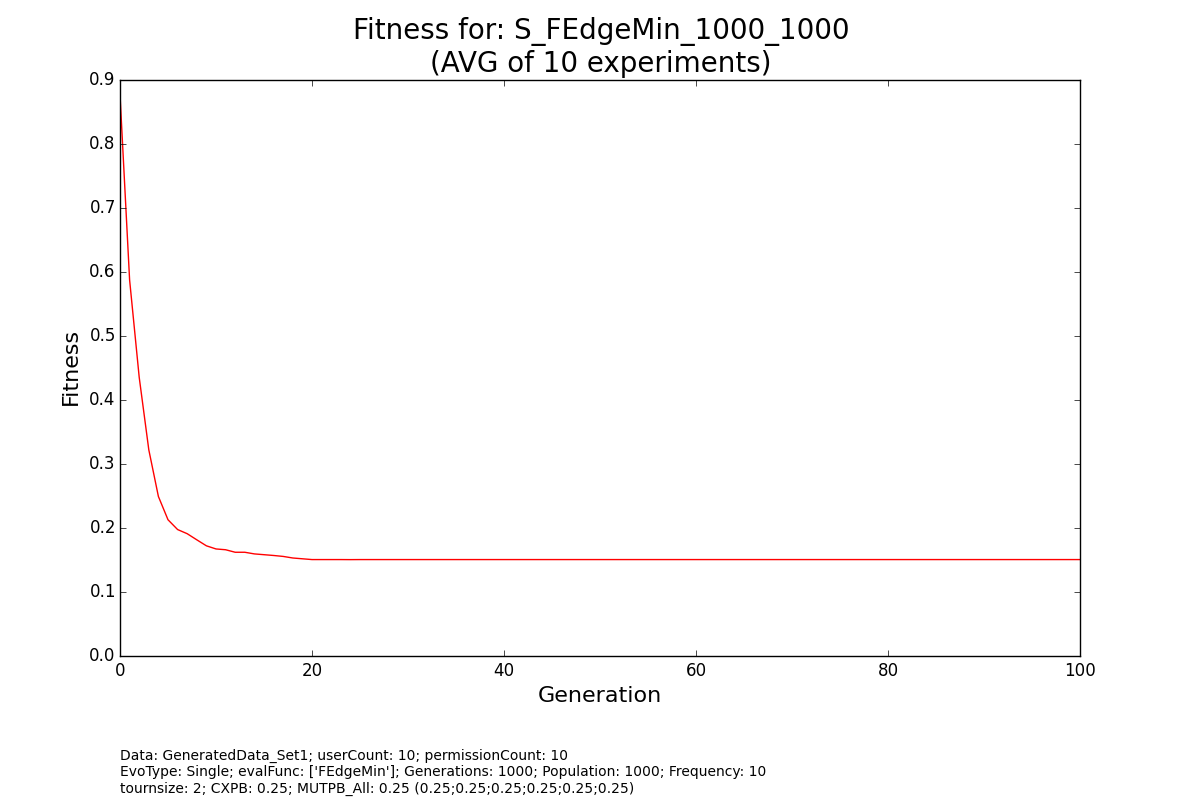
\includegraphics[scale=0.4, trim=0cm 2cm 0cm 0cm, clip=true]{./Figures/exp2bFitness}
        \caption{EXPERIMENT 2b: Average minimum Fitness Graph of ten experiments with fitness function $F_{edge}^{min}$ and synthetic dataset 1}
    \label{fig:exp2bfitness}
    \end{figure}


\subsection{Experiment 3a}
    \begin{figure}[H]
        \centering
        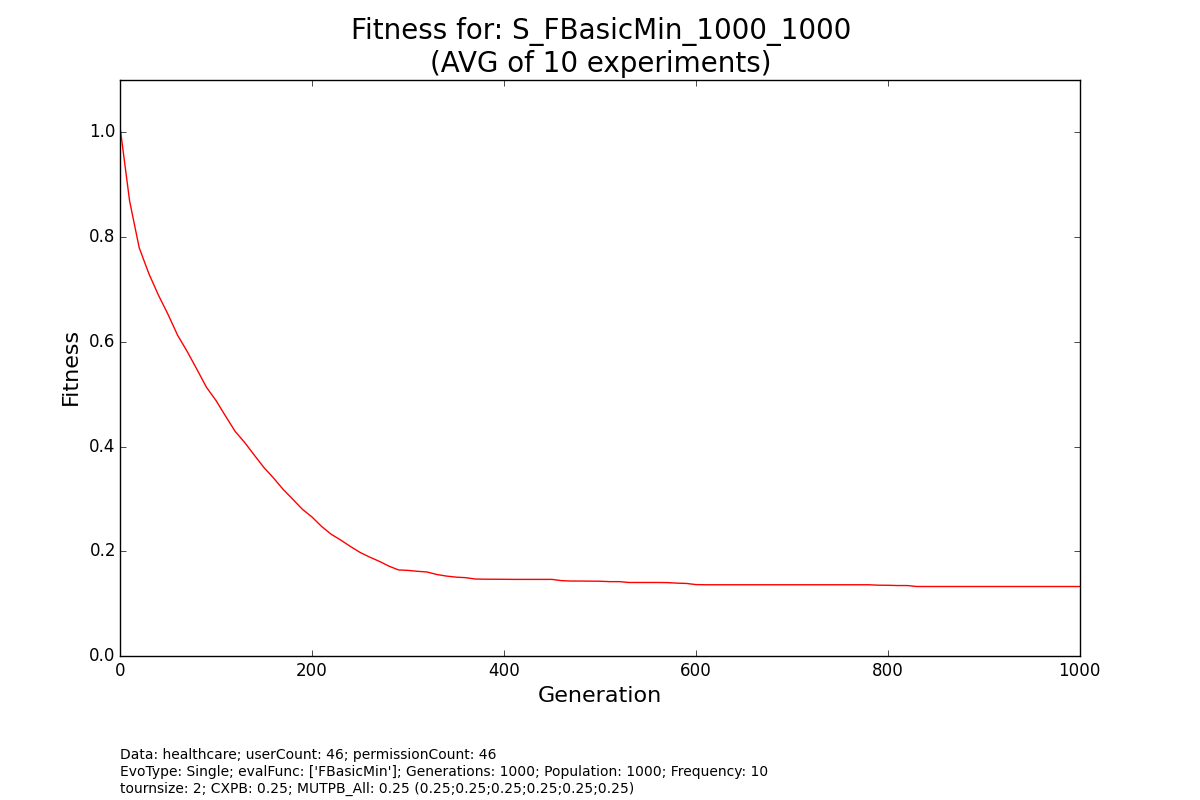
\includegraphics[scale=0.4, trim=0cm 2cm 0cm 0cm, clip=true]{./Figures/exp3aFitness}
        \caption{EXPERIMENT 3a: Average minimum Fitness Graph of ten experiments with fitness function $F_{basic}^{min}$ and healthcare dataset}
    \label{fig:exp3afitness}
    \end{figure}

    
\subsection{Experiment 3b}
    \begin{figure}[H]
        \centering
        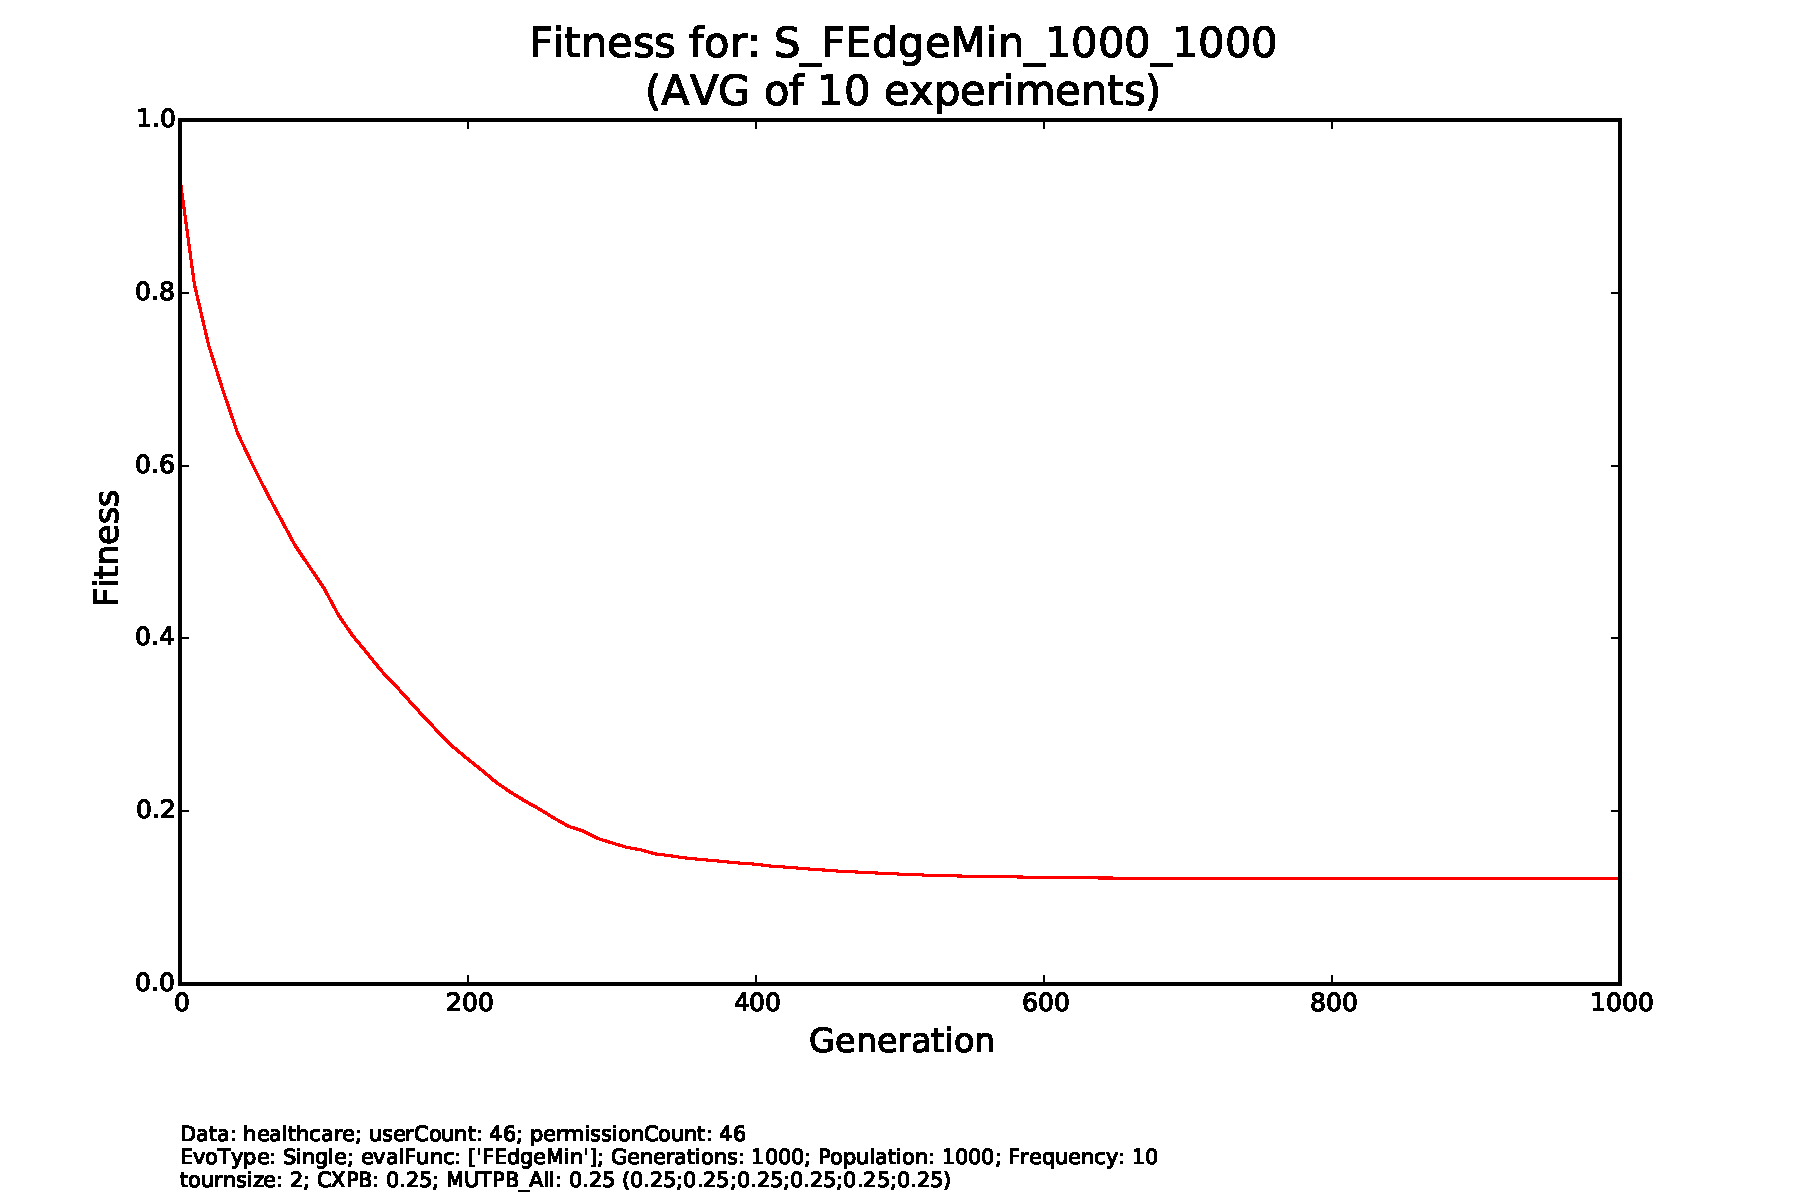
\includegraphics[scale=0.4, trim=0cm 2cm 0cm 0cm, clip=true]{./Figures/exp3bFitness}
        \caption{EXPERIMENT 3b: Average minimum Fitness Graph of ten experiments with fitness function $F_{edge}^{min}$ and healthcare dataset}
    \label{fig:exp3bfitness}
    \end{figure}

    
\subsection{Experiment 4a}
    \begin{figure}[H]
    	\centering
    	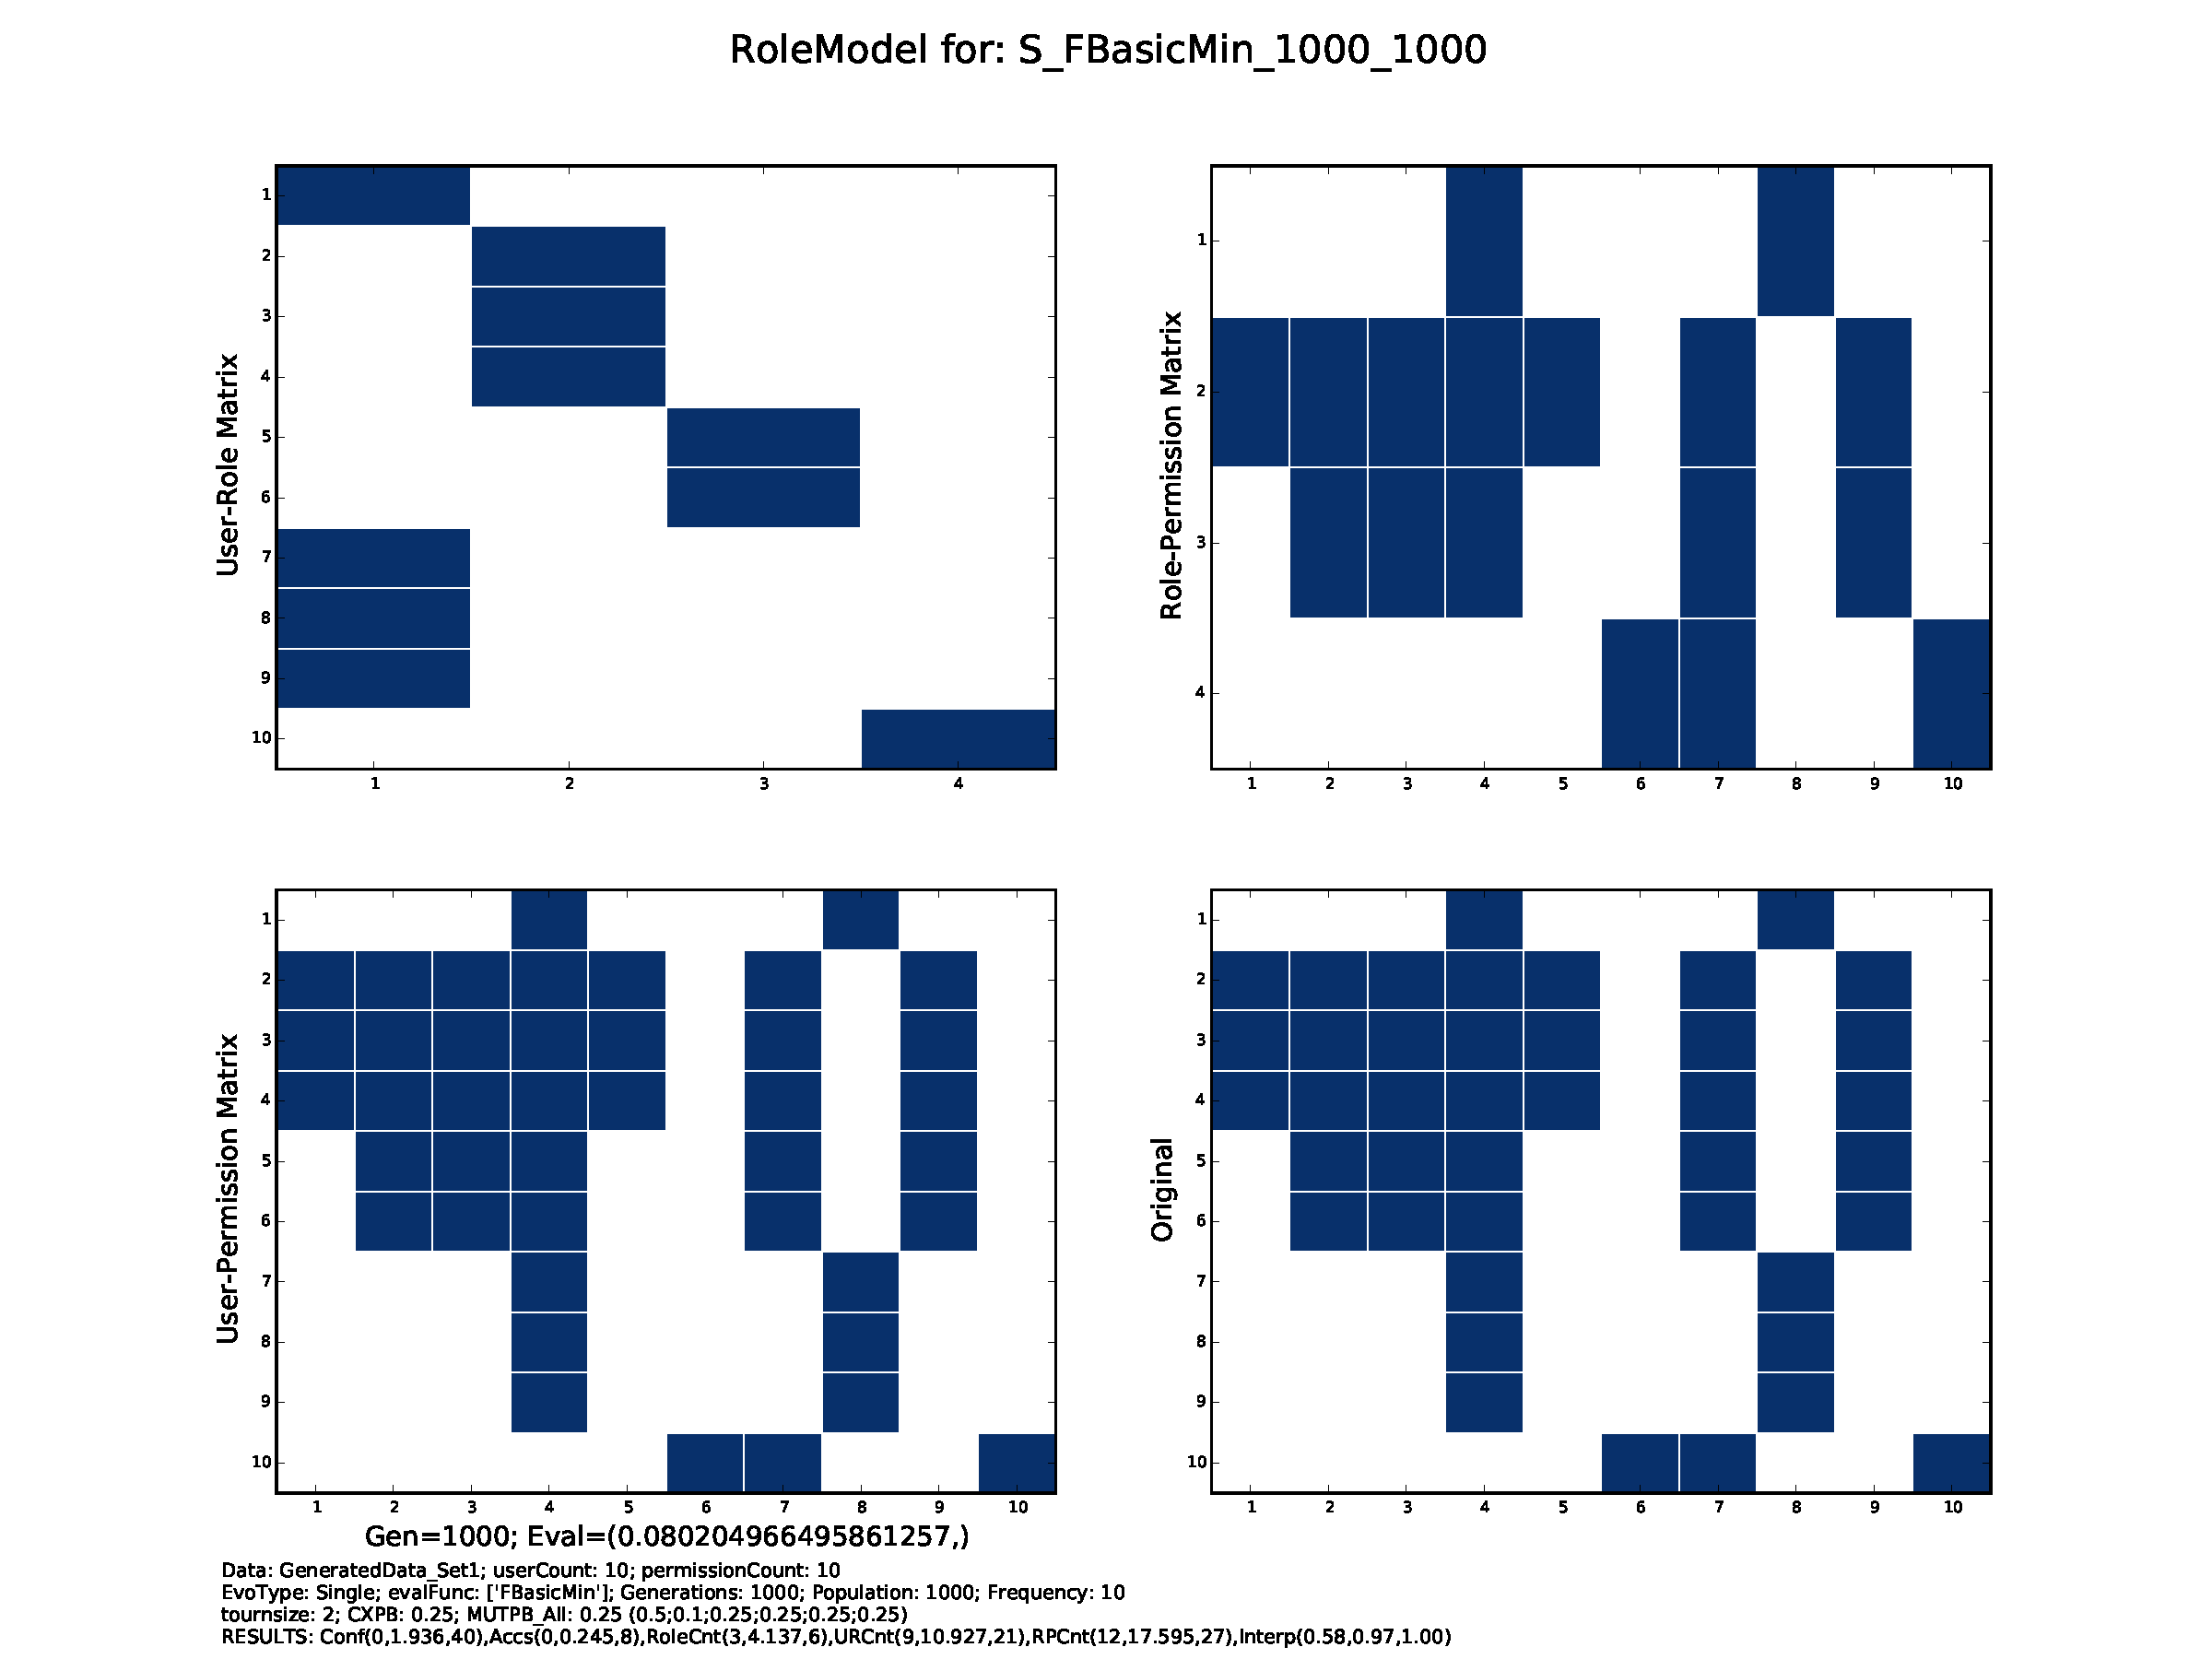
\includegraphics[scale=0.37, trim=4cm 2cm 4cm 2cm, clip=true]{./Figures/exp4aBasic_RM}
    	\caption{EXPERIMENT 4a: Example of fitness-optimal solution role model resulting of EvoRoleMiner with Fitness function $F_{basic}^{min}$ on synthetic dataset 1 with setup in table \ref{tab:setup3}. From u.l. to l.r.: User-Role Matrix, Role-Permission Matrix, Resulting User-Permission Matrix, Original User-Permission Matrix from Input. A blue box stands for an assignment. The darker the blue the more usre-role- and role-permission assignments causing the user-permission assignment.}
    	\label{fig:exp4aBasic_RM}
    \end{figure}

\subsection{Experiment 4b}
	\begin{figure}[H]
		\centering
		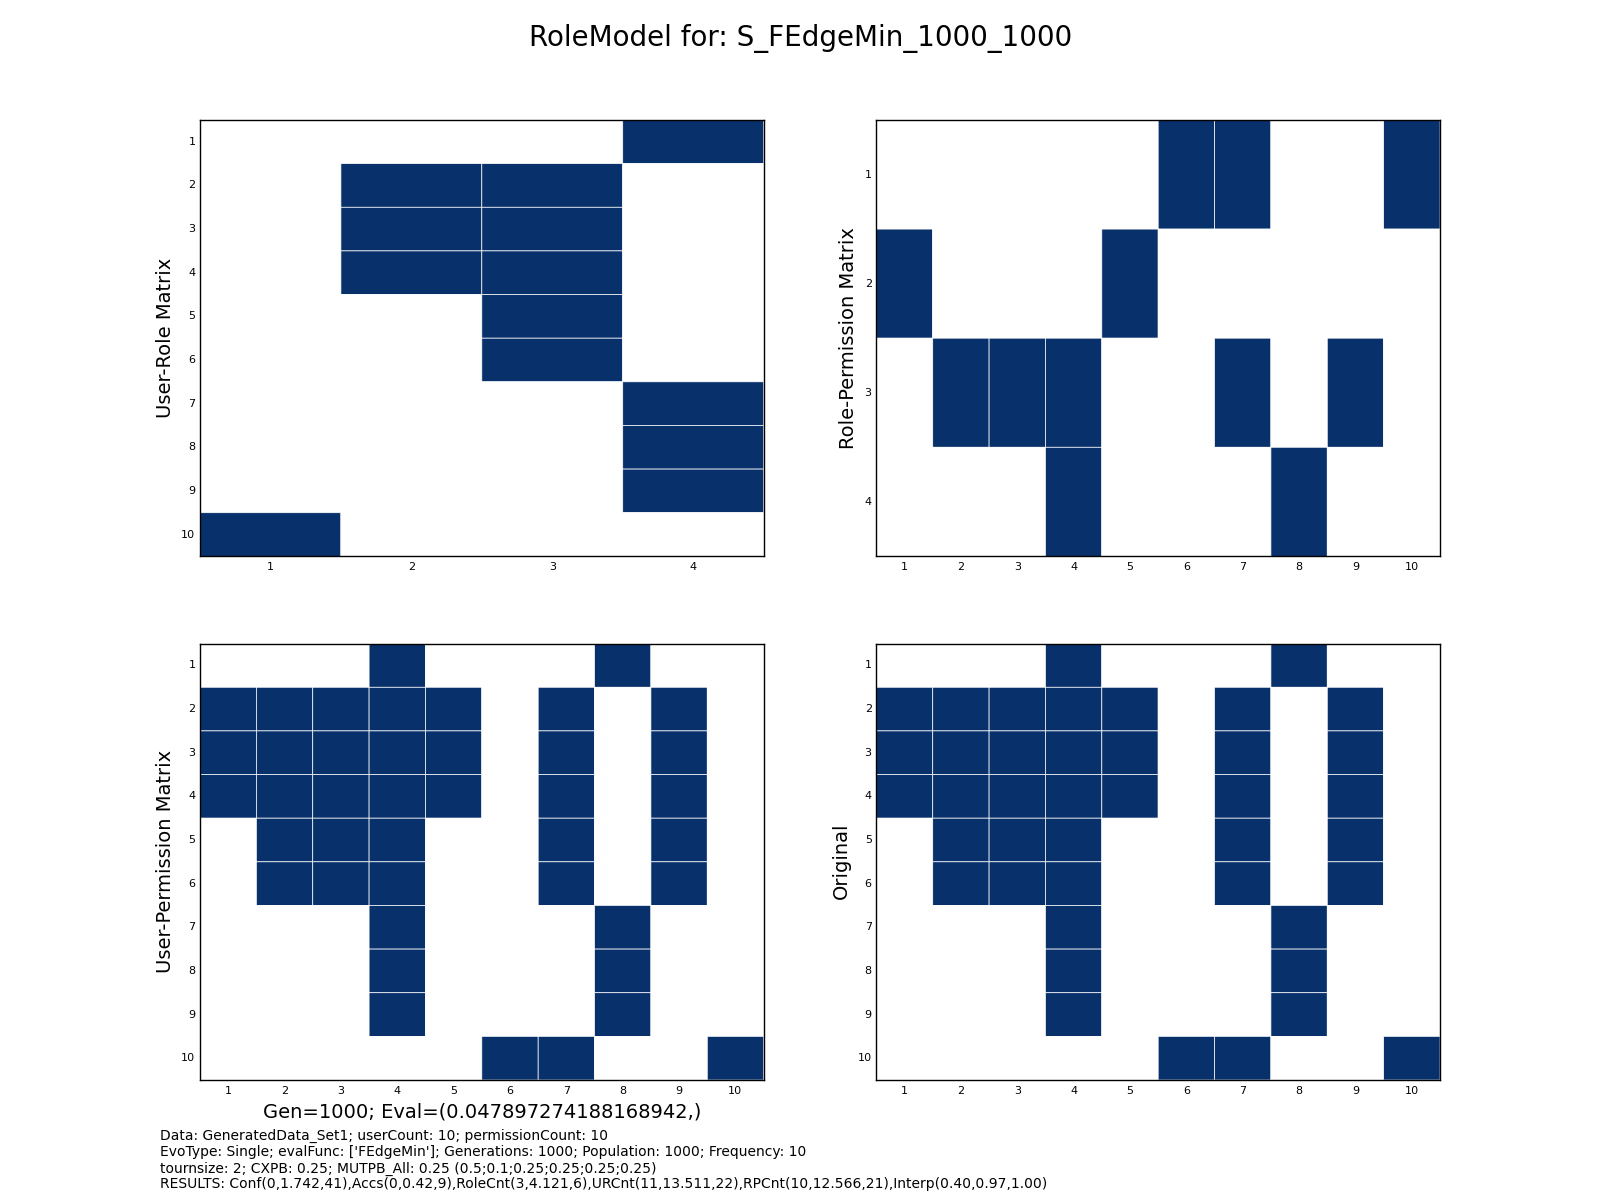
\includegraphics[scale=0.37, trim=4cm 2cm 4cm 2cm, clip=true]{./Figures/exp4bEdge_RM}
		\caption{EXPERIMENT 4a: Example of fitness-optimal solution role model resulting of EvoRoleMiner with Fitness function $F_{edge}^{min}$ on synthetic dataset 1 with setup in table \ref{tab:setup3}. From u.l. to l.r.: User-Role Matrix, Role-Permission Matrix, Resulting User-Permission Matrix, Original User-Permission Matrix from Input. A blue box stands for an assignment. The darker the blue the more usre-role- and role-permission assignments causing the user-permission assignment.}
		\label{fig:exp4bEdge_RM}
	\end{figure}


\subsection{Experiment 5a}

\subsection{Experiment 5b}